\documentclass[bachelor, och, referat]{SCWorks}
% параметр - тип обучения - одно из значений:
%    spec     - специальность
%    bachelor - бакалавриат (по умолчанию)
%    master   - магистратура
% параметр - форма обучения - одно из значений:
%    och   - очное (по умолчанию)
%    zaoch - заочное
% параметр - тип работы - одно из значений:
%    referat    - реферат
%    coursework - курсовая работа (по умолчанию)
%    diploma    - дипломная работа
%    pract      - отчет по практике
% параметр - включение шрифта
%    times    - включение шрифта Times New Roman (если установлен)
%               по умолчанию выключен

\usepackage{subfigure}
\usepackage{tikz,pgfplots}
\pgfplotsset{compat=1.5}
\usepackage{float}

%\usepackage{titlesec}
\setcounter{secnumdepth}{4}
%\titleformat{\paragraph}
%{\normalfont\normalsize}{\theparagraph}{1em}{}
%\titlespacing*{\paragraph}
%{35.5pt}{3.25ex plus 1ex minus .2ex}{1.5ex plus .2ex}

\titleformat{\paragraph}[block]
{\hspace{1.25cm}\normalfont}
{\theparagraph}{1ex}{}
\titlespacing{\paragraph}
{0cm}{2ex plus 1ex minus .2ex}{.4ex plus.2ex}

% --------------------------------------------------------------------------%


\usepackage[T2A]{fontenc}
\usepackage[utf8]{inputenc}
\usepackage{graphicx}
\graphicspath{ {./images/} }
\usepackage{tempora}

\usepackage[sort,compress]{cite}
\usepackage{amsmath}
\usepackage{amssymb}
\usepackage{amsthm}
\usepackage{fancyvrb}
\usepackage{listings}
\usepackage{listingsutf8}
\usepackage{longtable}
\usepackage{array}
\usepackage[english,russian]{babel}

% \usepackage[colorlinks=true]{hyperref}
\usepackage{url}


\newcommand{\eqdef}{\stackrel {\rm def}{=}}

\renewcommand\theFancyVerbLine{\small\arabic{FancyVerbLine}}

\newtheorem{lem}{Лемма}

\begin{document}

% Кафедра (в родительном падеже)
\chair{}

% Тема работы
\title{Современные средства хранения информации на жестких магнитных дисках}

% Курс
\course{1}

% Группа
\group{131}

% Факультет (в родительном падеже) (по умолчанию "факультета КНиИТ")
\department{факультета КНиИТ}

% Специальность/направление код - наименование
%\napravlenie{09.03.04 "--- Программная инженерия}
%\napravlenie{010500 "--- Математическое обеспечение и администрирование информационных систем}
%\napravlenie{230100 "--- Информатика и вычислительная техника}
%\napravlenie{231000 "--- Программная инженерия}
\napravlenie{090301 "--- Компьютерная безопасность}

% Для студентки. Для работы студента следующая команда не нужна.
\studenttitle{Студентов}

% Фамилия, имя, отчество в родительном падеже
\author{
    Гущина Андрея Юрьевича, \\
    Стаина Романа Игоревича, \\
    Улитина Ивана Владимировича 
}

% Заведующий кафедрой
% \chtitle{} % степень, звание
% \chname{}

%Научный руководитель (для реферата преподаватель проверяющий работу)
\satitle{доцент} %должность, степень, звание
\saname{О. В. Мещерякова}

% Руководитель практики от организации (только для практики,
% для остальных типов работ не используется)
% \patitle{к.ф.-м.н.}
% \paname{С.~В.~Миронов}

% Семестр (только для практики, для остальных
% типов работ не используется)
%\term{8}

% Наименование практики (только для практики, для остальных
% типов работ не используется)
%\practtype{преддипломная}

% Продолжительность практики (количество недель) (только для практики,
% для остальных типов работ не используется)
%\duration{4}

% Даты начала и окончания практики (только для практики, для остальных
% типов работ не используется)
%\practStart{30.04.2019}
%\practFinish{27.05.2019}

% Год выполнения отчета
\date{2020}

\maketitle

% Включение нумерации рисунков, формул и таблиц по разделам
% (по умолчанию - нумерация сквозная)
% (допускается оба вида нумерации)
% \secNumbering

\tableofcontents

% Раздел "Обозначения и сокращения". Может отсутствовать в работе


% Раздел "Определения". Может отсутствовать в работе
%\definitions

% Раздел "Определения, обозначения и сокращения". Может отсутствовать в работе.
% Если присутствует, то заменяет собой разделы "Обозначения и сокращения" и "Определения"
% \defabbr

% Раздел "Введение"
\intro

Мы живем в эпоху информационного Средневековья -- считают специалисты Ассоциации
сетевых технологий. Понятие ``Средние века'' характеризует этап развития 
носителей цифровой информации, находящийся в середине между «эпохой» малоемких
ненадежных дискет и ``веком'' сверхъемких долговечных накопителей будущего. 
Современные способы хранения данных еще далеки от совершенства -- большинство 
носителей имеет непродолжительный срок жизни, не превышающий 5-10 лет. 

Перед тем как рассказать о современных средствах хранения информации на жестких 
магнитных дисках, полагаю, для начала стоит дать определение словосочетанию 
``жесткий магнитный диск'', понять, как он работает, а также разобрать, из чего 
же он сделан.

\section{Жесткий магнитный диск}

\subsection{Краткий обзор}

Жесткий диск (или, как его еще иногда называют, винчестер или НЖМД) -- 
накопитель на жестких магнитных дисках (оригинальное название в английском 
языке -- hard (magnetic) disk drive, HDD, HMDD) -- запоминающее устройство 
(устройство хранения информации, накопитель) произвольного доступа, основанное 
на принципе магнитной записи. Является основным накопителем данных в 
большинстве компьютеров. 

\begin{figure}[H]
    \centering
    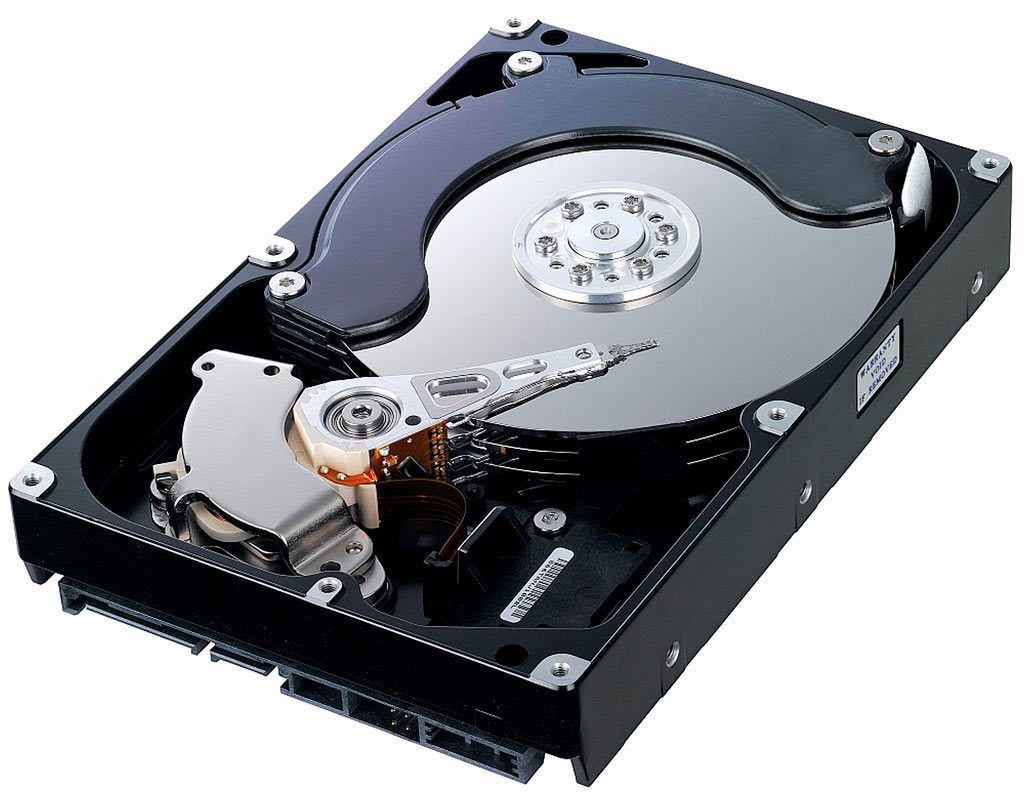
\includegraphics[width=0.7\textwidth]{hdd.png}
    \caption{}
    \label{}
\end{figure}

В отличие от гибкого диска (дискеты), информация в НЖМД записывается на жёсткие 
(алюминиевые или стеклянные) пластины, покрытые слоем ферромагнитного 
материала, чаще всего диоксида хрома -- магнитные диски. В НЖМД используется 
одна или несколько пластин на одной оси. Считывающие головки в рабочем режиме 
не касаются поверхности пластин благодаря прослойке набегающего потока воздуха, 
образующейся у поверхности при быстром вращении. Расстояние между головкой и 
диском составляет несколько нанометров (в современных дисках около 10 нм), а 
отсутствие механического контакта обеспечивает долгий срок службы устройства. 
При отсутствии вращения дисков головки находятся у шпинделя или за пределами 
диска в безопасной ``парковочной'' зоне, где исключен их нештатный контакт с 
поверхностью дисков. 

Также, в отличие от гибкого диска, носитель информации обычно совмещают с 
накопителем, приводом и блоком электроники. Такие жёсткие диски часто 
используются в качестве несъемного носителя информации.

Со второй половины 2000-х годов получили распространение более производительные 
твердотельные накопители, вытесняющие дисковые накопители из ряда применений 
несмотря на более высокую стоимость единицы хранения; жёсткие диски при этом, 
по состоянию на середину 2010-х годов, получили широкое распространение как 
недорогие и высокоёмкие устройства хранения как в потребительском сегменте, 
так и корпоративном.

Вследствие наличия термина логический диск, магнитные диски (пластины) жёстких 
дисков, во избежание путаницы, называются физический диск, сленговое -- блин. 
По этой же причине твердотельные накопители иногда называются жёсткий диск SSD, 
хотя магнитные диски и подвижные устройства в них отсутствуют.

\subsection{Винчестер}

По одной из версий, название ``винчестер'' (англ. Winchester) накопитель 
получил благодаря работавшему в фирме IBM Кеннету Хотону (англ. Kenneth E. 
Haughton), руководителю проекта, в результате в 1973 году был выпущен 
жёсткий диск модели 3340, впервые объединивший в одном неразъёмном 
корпусе пластины диска и считывающие головки. При его разработке инженеры 
использовали краткое внутреннее название ``30-30'', что означало два модуля 
(в максимальной компоновке) по 30 мегабайт каждый, что по созвучию совпало 
с обозначением популярного охотничьего оружия — винтовки Winchester Model 
1894, использующего винтовочный патрон .30-30 Winchester. Также существует 
версия, что название произошло исключительно из-за названия патрона, 
также выпускавшегося Winchester Repeating Arms Company, первого созданного 
в США боеприпаса для гражданского оружия ``малого'' калибра на бездымном порохе,
который превосходил патроны старых поколений по всем показателям и немедленно 
завоевал широчайшую популярность. В Европе и США название ``винчестер'' вышло 
из употребления в 1990-х годах, в русском же языке сохранилось и получило 
полуофициальный статус, а в компьютерном сленге сократилось до слова ``винт'' 
(иногда ``винч'').


\section{История жёстких дисков}

Первый жесткий диск это продукт, который разработала компания IBM в 1956 году, 
и вошел он в историю как начало компьютерной индустрии.

\begin{figure}[H]
    \centering
    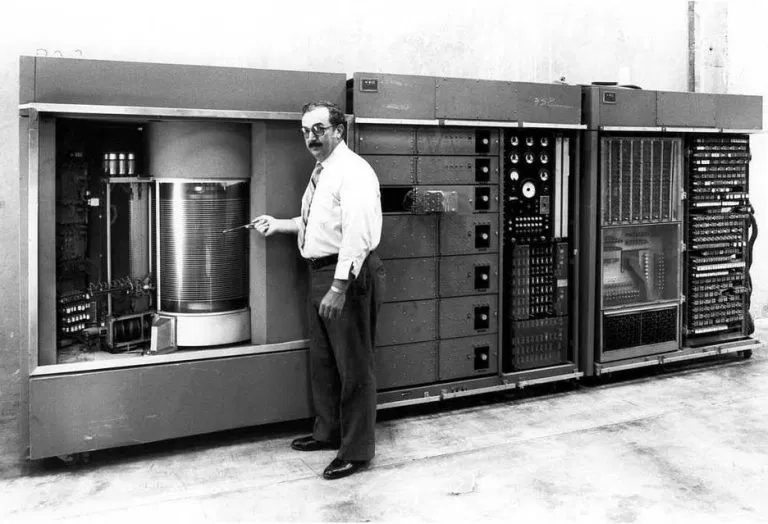
\includegraphics[width=0.7\textwidth]{ibm350.png}
    \caption{Дисковод IBM 350 состоял из 50 пластин диаметром 24 дюйма -- все имело невероятную емкость 5 МБ}
    \label{}
\end{figure}

IBM 350 оказался настоящим прорывом в области хранения данных из которого и 
началась история HDD. Благодаря использованию 50 магнитных пластин диаметром 
24 дюйма, вращающихся со скоростью 1200 оборотов в минуту, он практически во 
всех отношениях шел впереди популярных тогда решений.

\begin{figure}[H]
    \centering
    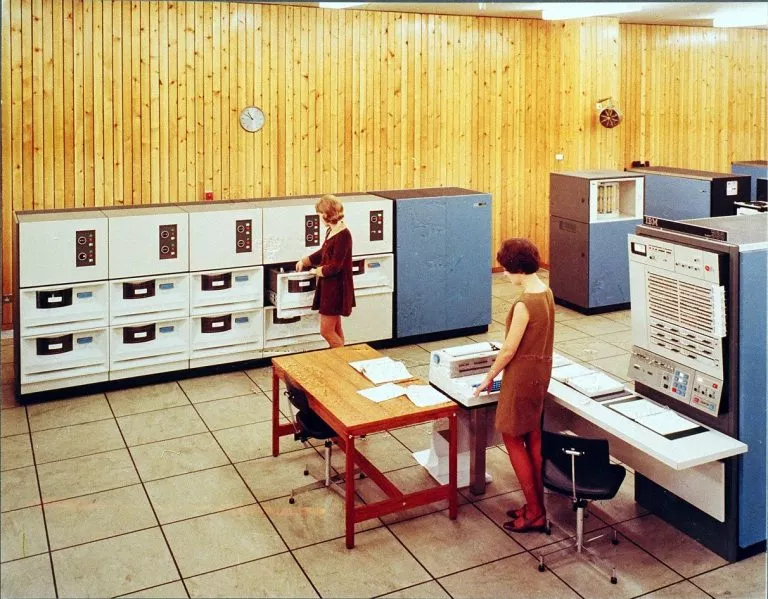
\includegraphics[width=0.6\textwidth]{ibm2310.png}
    \caption{1965 год -- IBM 2310}
    \label{}
\end{figure}

В 1956-61 годы компания IBM выпустила более 1000 компьютеров IBM 305 RAMAC, 
оборудованных дисковыми накопителями. Несмотря на то, что прошло уже 60 лет, 
современные жесткие диски все еще работают по тому же принципу что и IBM 350.

Вскоре, основываясь на опыте с модели 350, компания IBM начала создавать все 
более и более мощные конструкции. Жесткий диск IBM 1301 с 1961 года мог хранить 
28 МБ данных на 25 дисках. Каждый из них имел специальную головку, что позволило 
сократить время доступа к данным от 600 до 180 мс. В 1965 году был создан модуль 
хранилища IBM 2310, использующий сменные картриджи объемом 1 МБ.

\begin{figure}[H]
    \centering
    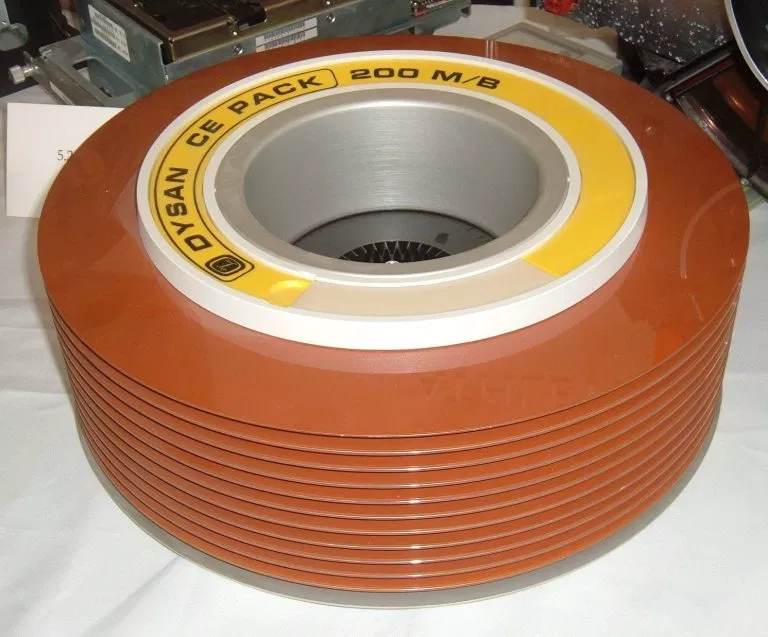
\includegraphics[width=0.6\textwidth]{ibm3300.png}
    \caption{1970 год -- IBM 3300}
    \label{}
\end{figure}

В 1970 году дебютировала на рынке модель IBM 3300 с поворотным механизмом 
коррекции ошибок. Система состояла из двух модулей со сменными носителями, и 
стоила в сегодняшнем эквиваленте около 400 тыс. долларов. Один носитель данных 
(так называемый Disk Pack) содержит в себе 11 дисков диаметром 14-дюймов и имел 
емкость 100 МБ, а начиная с 1974 года – 200 МБ. Модули можно было комбинировать 
друг с другом, так что жесткие диски первый раз стали в состоянии предложить 
гигабайтовые емкости. По-прежнему серьезным препятствием были 
большие размеры привода.

Магнитные диски HDD в первый раз встретились с реальной конкуренцией в 1976 
году. Компания Dataram представила тогда привод Bulk Core, который сегодня 
считается родоначальником дисков SSD (Solid State Drive). В них использовалась 
так называемая ферритовая память, характерной чертой которой было отсутствие 
механических элементов. Время доступа к данным, составляло всего 2мс. Решение 
было интересным, но также очень дорогим и непрактичным. Если перевести цену 
памяти Bulk Core на нынешние условия, то 1 ТБ дискового пространства обойдется 
около 1,6 млрд долларов. Билл Гейтс на все свое состояние сможет купить около 
49 ТБ пространства для хранения данных. Немного, как для самого богатого 
человека в мире.

\begin{figure}[H]
    \centering
    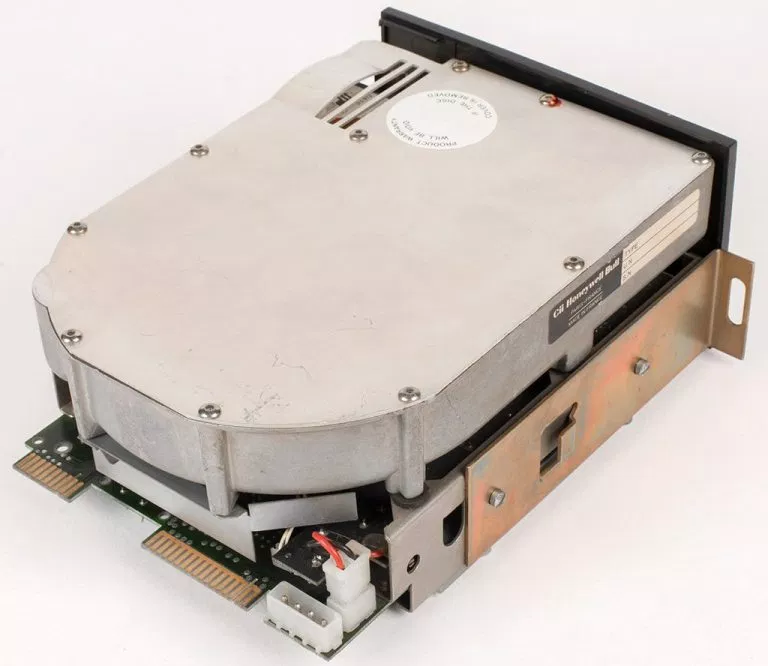
\includegraphics[width=0.7\textwidth]{st506.png}
    \caption{1980 год -- диск ST-506}
    \label{}
\end{figure}

Настоящая революция в индустрии жестких дисков состоялась только в 1980 году, 
когда компания Shugart Technology представила диск ST-506. Он обеспечивал объем 
такой же, как IBM 350 в 1956 году, то есть 5 МБ. Однако имел ``миниатюрный'' 
формат в 5,25 дюйма и весил ``всего'' 3,2 кг. Его можно было уместить в первых 
корпусах ПК. ST-506 одержал рыночный успех, а компания Shugart сегодня известна 
как Seagate.

Еще одним важным новшеством на рынке была премьера диска Rodime RO352 в 1983 
году. Эта, несуществующая уже шотландская компания умудрилась уместить 
накопитель HDD объемом 10 МБ в 3,5-дюймовом корпусе. Так родился стандарт, 
который до сегодняшних дней используют все модели жестких дисков.

80-е годы на рынке жестких дисков стали периодом миниатюризации и 
стандартизации. Появились интерфейсы SCSI и IDE, а японский концерн Toshiba во 
второй половине десятилетия разработал технологию памяти полупроводниковых 
NAND flash.

В 1988 году на рынке дебютировал первый жесткий диск в формате 2,5 дюйма -- 
PrairieTek 220 емкостью 20 МБ. Так же, как Rodime RO352, он считался важным 
прорывом в эволюции HDD. Десять лет спустя диски 2,5 дюйма стали массово 
использоватся в ноутбуках. В 2006 году формат 2,5 дюйма стал стандартом на рынке
жестких дисков с интерфейсом SATA.

\begin{figure}[H]
    \centering
    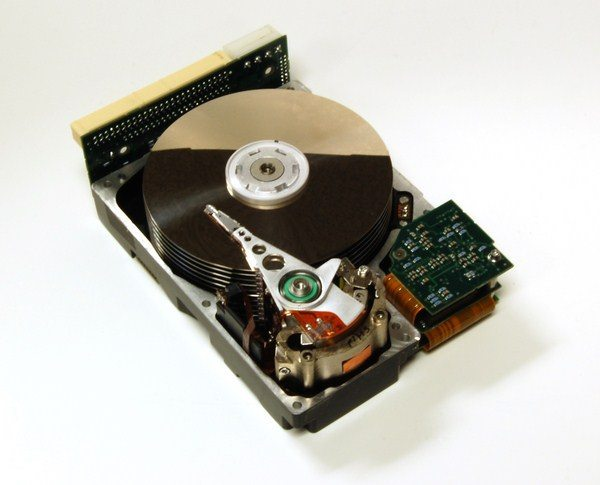
\includegraphics[width=0.7\textwidth]{seagate1992.png}
    \caption{1992 год -- Seagate представила диск емкостью 2,1 ГБ}
    \label{}
\end{figure}

В начале 90-х развитие жестких дисков ускорилось в результате бума на ПК. IBM 
первую гигабайтную модель HDD вывел на рынок уже в 1991 году. Это была модель 
0663 Corsair — 3,5-дюймовая конструкция с 8 дисками. Год спустя компания 
Seagate представила диск емкостью 2,1 ГБ с дисками, вращающимися со скоростью 
7200 оборотов в минуту.

В 1995 году израильская компания M-Systems разработала первый диск FFD 
(Fast Flash Disk), который своим форматом 3,5 дюйма был похож на классические 
жесткие диски, однако при этом имел основу NAND. Он не имел никаких движущихся 
элементов, предлагал очень короткое время доступа и, что особенно важно, 
считался исключительно прочным и надежным. Решения, рожденные под аббревиатурой 
FFD стоили кучу денег, но пришлись по вкусу военным. Также они стали 
использоваться для регистраторов полета, в народе называемые черными ящиками.

\begin{figure}[H]
    \centering
    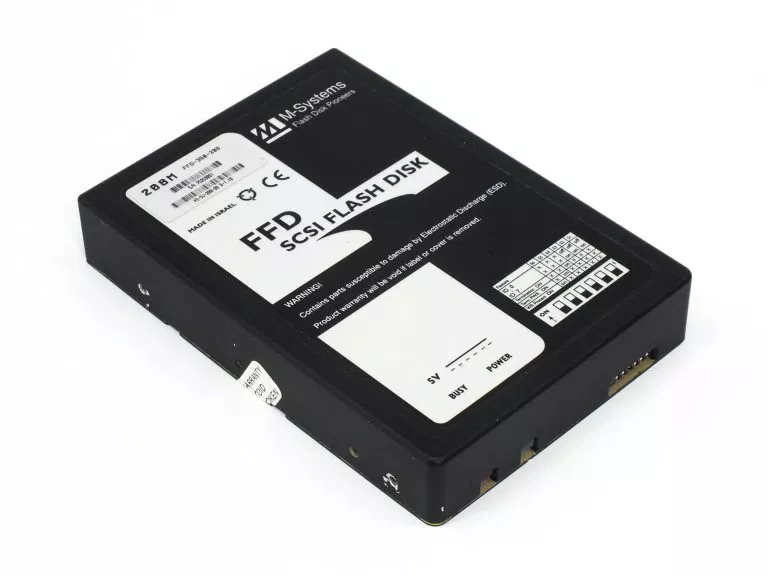
\includegraphics[width=0.7\textwidth]{fdd.png}
    \caption{1995 год -- первый диск FFD}
    \label{}
\end{figure}

Конец XX века это времена пластин, вращающихся с огромными скоростями. В 1996 
году компания Seagate создала жесткие диски семейства Cheetah. Первые модели 
разгонялись до 10000 оборотов в минуту, а в моделях Cheetah X15 с 2000 года 
диски вращались со скоростью 15000 об. Это были самые быстрые жесткие диски с 
интерфейсом IDE. Оценили их за эффективность, но не одобрили из-за 
производимого высокого шума.

Можно с уверенностью сказать, что XXI век наступил для жестких дисков в конце 
2002 года, наряду с выпуском универсального интерфейса SATA. Новое поколение 
накопителей HDD полюбили игроки. Особенно те, которые могли позволить себе 
покупку двух дисков и соединение их в массив RAID0. Разъем SATA быстро стал 
стандартом, и так же быстро начал развиваться. В 2004 году дебютировала вторая 
генерация (SATA II 3 Gb/s), а спустя пять лет — третья (SATA III 6 Gb/s). Когда 
в 2006 году начали дешеветь дорогие раньше флеш-памяти NAND, HDD заимели 
серьезного конкурента в виде первых SSD.


\section{Устройство жесткого диска}

Накопитель на жестких магнитных дисках состоит из одной или нескольких пластин 
с магнитным слоем, головок, позиционирующего устройства, корпуса, а также 
контроллера. Пластины – основной элемент накопителя, на них размещается 
информация. Головки предназначены для чтения и записи информации на пластины. 
Позиционирующее устройство обеспечивает перемещение головок к нужному месту на 
поверхности пластин. Корпус служит для крепления остальных элементов 
конструкции, а также для защиты пластин и головок от механических повреждений 
и пыли. Контроллер управляет всеми электрическими и электромеханическими узлами 
накопителя и обеспечивает передачу информации из компьютера и обратно.

\begin{figure}[H]
    \centering
    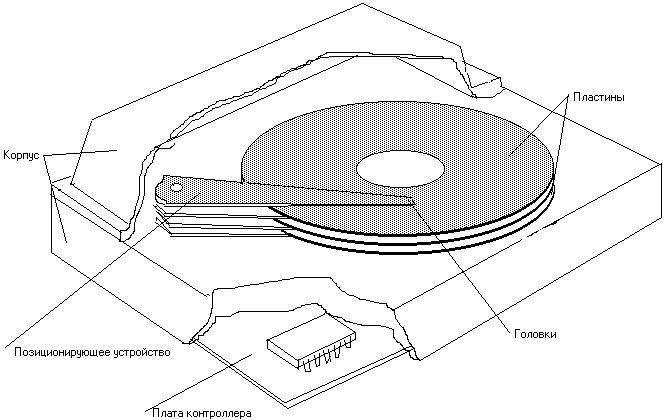
\includegraphics[width=0.6\textwidth]{org_hdd.png}
    \caption{}
    \label{}
\end{figure}

\subsection{Геометрия жесткого диска}

Пластины накопителя изготовляются из металла или стекла и имеют с одной или 
обеих сторон магнитный слой, на который и происходит запись информации. Сторона 
пластины с нанесенным магнитным слоем называется рабочей поверхностью. 
Поверхности пластин тщательно отполированы и покрыты ферромагнитным слоем. 
Материал покрытия и количество слоев (магнитный слой может состоять из 
нескольких слоев разных материалов) может быть различным для разных накопителей.
На каждую рабочую поверхность приходится по одной головке (на самом деле в 
современных накопителях для увеличения плотности записи применяются отдельные 
головки записи и чтения, изготовленные по различным технологиям). Поверхность 
пластины разбивается на тонкие концентрические кольцевые зоны, называемые 
дорожками. А каждая дорожка, в свою очередь, делится на несколько участков, 
получивших названия секторов. Сектор можно условно разделить на две области: 
область данных и область служебной информации. Служебная информация 
записывается на пластину один раз на заводе-изготовителе и в дальнейшем не 
подлежит изменению. Служебная область включает уникальный адрес сектора в 
накопителе, по которому его опознает контроллер при записи или считывании 
информации. Область данных содержит полезную информацию, записываемую на 
накопитель. Эта область может быть многократно изменена в период эксплуатации. 
Объем области данных несколько превосходит информационную емкость сектора за 
счет дополнительной информации – для верификации и, возможно, исправления 
ошибок. Область данных сектора может быть обновлена только целиком. Т.е. на 
накопитель нельзя записать один или десять байт – только сектор целиком. Все 
головки перемещаются синхронно, и этот процесс занимает некоторое время. 
Совокупность дорожек на разных пластинах доступных одновременно при неизменном 
положении головок называется цилиндром. С точки зрения производительности 
дисковой системы целесообразно последовательные данные располагать в пределах 
одного цилиндра.

\begin{figure}[H]
    \centering
    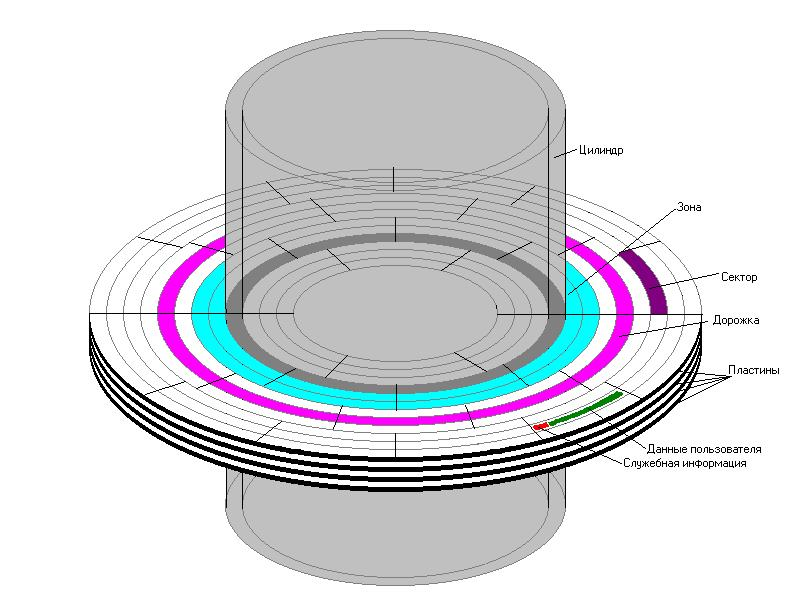
\includegraphics[width=0.7\textwidth]{geom_hdd.png}
    \caption{}
    \label{}
\end{figure}

В старых накопителях все дорожки содержали одинаковое количество секторов. В 
этом случае уникальный адрес каждого сектора (т.е. минимальной порции 
информации, хранимой на накопителе) мог быть задан тремя числами: номерами
цилиндра, головки и сектора. Таким образом, на жестком диске была введена 
трехмерная система координат, очень напоминающая цилиндрическую в трехмерном 
пространстве: радиусу соответствует номер цилиндра, высоте – номер головки, 
а углу – номер сектора.

Если представить такую конструкцию в декартовой системе координат (например, 
считать, что наш ``диск'' собран из нескольких плат с флэш-памятью), то она будет 
представлять собой по форме параллелепипед, разбитый на ячейки - сектора.

Однако, при такой разметке жесткого диска плотность записи на внешних дорожках 
оказывается примерно втрое ниже, чем на внутренних (одно и то же количество 
информации на втрое превосходящую длину дорожки). Поэтому в современных 
накопителях используется так называемая зонная запись, при которой поверхность 
пластин разделяется вдоль радиуса на несколько зон (обычно около десятка), в 
каждой из которых количество секторов на дорожку постоянно, однако, это 
количество меняется от зоны к зоне. На внешних дорожках размещается больше 
секторов, чем на внутренних. Это позволяет увеличить информационную емкость 
накопителя примерно вдвое без изменения максимальной плотности записи. Но, 
будучи представленной в декартовой геометрии, такая фигура будет иметь 
достаточно сложную форму, с которой не сможет работать BIOS. Поэтому из всего 
многообразия интерфейсов жестких дисков (ST506/412, ESDI, IDE, SCSI) остались 
только два последних, отличающихся наибольшей ``интеллектуальностью'', что 
выражается в способности осуществлять такое ``преобразование координат'' при 
котором фигура неправильной формы превращается в аккуратный "кирпичик". Заодно 
такое преобразование позволяет обойти или, по крайней мере, несколько смягчить 
ограничения, налагаемые BIOS на максимальные значения некоторых параметров. 
Например, BIOS не может работать более чем с 63 секторами на дорожке, в то 
время как на современных дисках их примерно на порядок больше. В то же время, 
BIOS может ``думать'', что у жесткого диска 16 или даже 255 головок, в то время 
как в реальных накопителях это число лежит в пределах, как правило, от 1 до 6.

\begin{figure}[H]
    \centering
    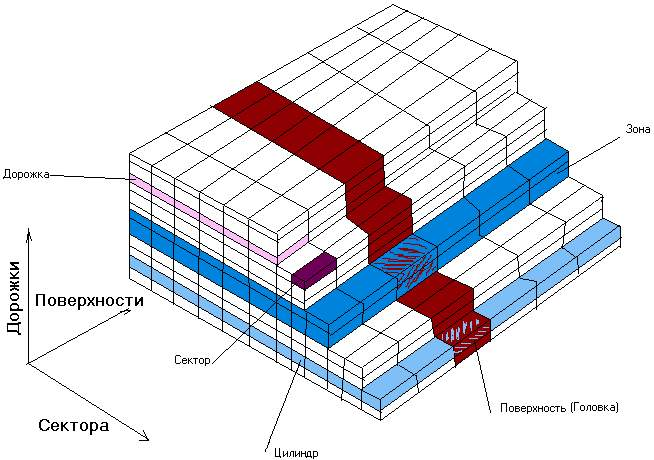
\includegraphics[width=0.7\textwidth]{layers_hdd.png}
    \caption{}
    \label{fig:layers}
\end{figure}
  
Естественно, зонная запись, т.е. различное количество секторов на разных 
дорожках при постоянной скорости вращения ведет к тому, что скорость обмена 
данными будет зависеть от номера цилиндра.

\begin{figure}[H]
    \centering
    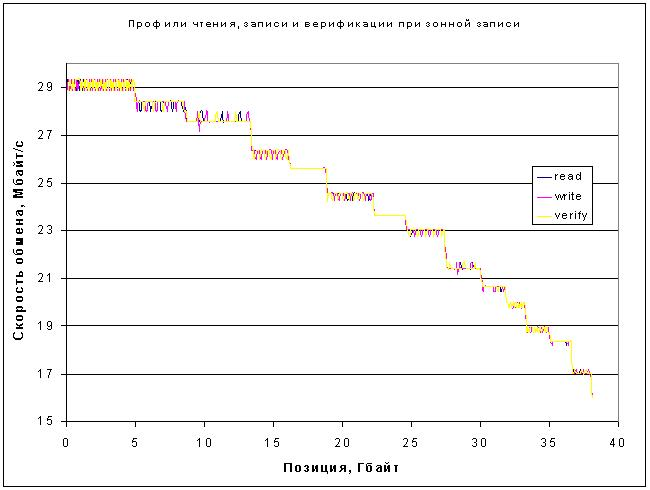
\includegraphics[width=0.6\textwidth]{graph1.png}
    \caption{}
    \label{}
\end{figure}

\subsection{Ограничения на объем}

В свое время при разработке первых версий BIOS для IBM PC было решено ограничить
количество секторов и цилиндров одним 16-разрядным числом, при этом для сектора 
отводилось 6 разрядов (максимальный номер 63), а для цилиндра -- 10 
(максимальный номер – 1023). Для номера головки BIOS было отведено 8 разрядов 
(максимальное число – 255). Но интерфейс IDE допускал не более 16 головок, что 
при размере сектора 512 байт по сумме всех ограничений давало верхнюю границу в 
504 Мбайта (528 482 304 байта). Разрешение этой проблемы заключалось во введении
режима LBA, т.е. ``переносе'' неиспользуемых разрядов номера головки для адресации
номера цилиндра. Такое решение требовало одновременно как аппаратной (со стороны 
IDE-контроллера), так и программной (со стороны BIOS) поддержки. Одновременно 
оказалась исчерпанной пропускная способность шины ISA. Поэтому слегка 
переработанный контроллер (теперь уже с интерфейсом, называемым EIDE) стали 
помещать на системную плату, т. е. туда же, где располагалась микросхема BIOS с 
поддержкой новых возможностей.

Но только была преодолена эта граница, как выяснилось, что следующее ограничение 
связано уже с файловой системой FAT16 – размер логического диска не может быть 
больше 2 Гбайт (точнее 2047 Мбайт). При этом место на жестком диске расходуется 
на редкость неэффективно.

Введение FAT32 позволило преодолеть этот предел, однако вскоре снова ``вылезла''
проблема BIOS -- на полный адрес сектора отводилось 24 разряда, и адресация 
более 8 Гбайт (точнее 7.85 Гбайт) дисковой памяти при 512-байтных секторах 
оказалась невозможной. Пришлось ввести новые функции BIOS для большинства 
дисковых операций. Теперь лимит составляет 64 разряда, что соответствует 
8 млрд. Тбайт, так что пока есть некоторый запас по времени. Кроме того 
оговорено, что нумерации подлежат блоки, а не сектора. Пока 1 блок равен 1 
сектору, но как только объем накопителей приблизится к указанному лимиту, 
появится некоторый резерв за счет увеличения размера блока.

Кроме того, так как с введением зонной записи привязка к физической структуре 
накопителя, выраженная в цилиндрах, секторах и головках, оказалась неактуальной, 
было решено отказаться от трехмерной системы координат и перейти к одномерной --
по абсолютному номеру сектора.

Теперь программных ограничений на рост объемов накопителей в ближайшее время не 
предвидится (но некоторые программы из-за содержащихся в них ошибок не могут 
работать с дисками объемом выше 32 или 64 Мбайт), хотя остаются определенные 
ограничения, связанные с аппаратурой, т.е. с физической организацией 
интерфейса IDE.


\section{Взаимодействие между пользователем и дисковым накопителем}

Рядовому пользователю было бы чрезвычайно обременительно следить за тем, какие сектора на его жестком диске уже заняты, и куда следует записывать новые данные. Чтобы облегчить ему эту работу служит операционная система (ОС), вводящая понятие файла и позволяющая работать с содержимым файла побайтно. Для этого ОС резервирует некоторое место на диске для своих нужд. Вот как выглядит дописывание нескольких байт к концу существующего файла в корневом каталоге с точки зрения ОС.

\begin{enumerate}
    \item Считать оглавление, содержащее нужный файл и поместить его в буфер №1,
    \item Считать таблицу FAT и поместить ее в буфер №2,
    \item В соответствии с FAT считать последний (неполный) сектор файла в буфер №3,
    \item Дописать часть требуемых байтов в буфер №3 до его заполнения,
    \item Вписать буфер №3 на его прежнее место на диске,
    \item Используя FAT, найти на диске свободный фрагмент,
    \item Вписать оставшиеся байты в буфер №4,
    \item Вписать содержимое буфера №4 в найденный свободный фрагмент диска,
    \item Внести изменения в FAT (в буфер №2) и вписать его на прежнее место на диске,
    \item Внести изменения длины файла в оглавление (буфер №1) и вписать его в прежнее место на диск.
\end{enumerate}

Это только самый простейший случай. Если файловая система предусматривает вложенные оглавления, защиту информации, разграничение доступа, откат и восстановление после сбоев, то список необходимых действий может увеличиться в несколько раз.

Мы уже говорили о том, что данные в накопителе адресуются через номер логического сектора или через тройку цилиндр-головка-сектор. Именно таким образом и обращается ОС к BIOS. Последний же, в свою очередь, должен сообщить ОС объем накопителя и, при необходимости, его геометрические характеристики, а также перевести запрос на операцию с определенным сектором в последовательность команд того или иного интерфейса. Для ОС тип интерфейса, ST512/412, ESDI. IDE, SCSI, USB, IEEE1394 или режим работы, PIO, UDMA неинтересны.

\section{Проблемы кластеризации}

Как мы видели, для работы с файлами постоянно требуется определенная информация по размещению их на диске. В приведенном выше случае это FAT. Для простоты ограничимся рассмотрением именно этого случая. Из 7 дисковых операций 3 относятся к FAT. Учитывая, что файловые операции, выполняемые с перемещением головки, происходят существенно медленнее операций без перемещения, получается, что хранение FAT в оперативной памяти увеличивает производительность файловой системы более чем вдвое. Но есть и явная отрицательная черта -- если перед выключением компьютера не привести в соответствие копию FAT, хранящуюся на диске, с копией в оперативной памяти, неизбежна потеря информации. Поэтому выключение компьютера кнопкой или тумблером на передней панели, как это практиковалось в DOS, уже становится неприемлемым.

При этом, если буфера для данных файла или каталога могли быть небольшими, в один сектор, то FAT иногда необходимо обрабатывать целиком, например, при поиске свободного фрагмента.

В FAT16 максимальное количество фрагментов, предназначенных для размещения файлов, составляет около 65 тысяч, а занимаемое таблицами место -- 128 Кбайт (64К 2-байтных слов). При распределении мест секторами максимальный объем диска составит, таким образом, 32 Мбайта (кто-то еще помнит, что реально было и такое ограничение на объем жесткого диска).

Для увеличения доступного ОС дискового пространства сектора пришлось объединять 
в кластеры, содержащие несколько секторов. Кроме того, очевидно, что при 
увеличении вдвое размера кластера вдвое же уменьшается размер FAT, а 
следовательно, как расход оперативной памяти, так и время поиска свободного 
места. Но увеличение размера кластеров ведет к неэффективному расходу дискового 
пространства. Мне когда-то попадалась аналогия распределения места на диске с 
необходимостью расплачиваться за любые товары только стодолларовыми купюрами: 
купил коробок спичек – и нет \$100, купил батон хлеба – еще сотню долой. 
Действительно, при записи даже одного байта расходуется целиком кластер. 
Например, при 32-Кбайтных кластерах (диск объемом 2 Гбайт) 1000 однобайтных 
файлов суммарной длиной менее Кбайта займут на диске место равное 32 Мбайтам.

Введение FAT32 отчасти устранило эту проблему, теперь для размещения аналогичного объема информации потребуется только 4 Мбайта. Но ничего бесплатного не бывает. Размер одного элемента FAT увеличился вдвое, а количество элементов -- в 8 раз, так что теперь объем таблиц для данного случая составит уже 2 Мбайта. Конечно, по нынешним меркам это немного, но если учесть, что объем накопителей может превышать сотню Гбайт, то окажется, что значительная доля оперативной памяти будет использована не для размещения данных пользователя, а для внутренних нужд ОС. Вспомним и о том, что для поиска свободного фрагмента на диске может потребоваться просмотреть значительную часть FAT, так что в попытках увеличить скорость работы дисковой системы мы одновременно увеличиваем нагрузку на центральный процессор и оперативную память, что ведет к снижению итоговой производительности.

В общем, прямого и простого пути к увеличению производительности не существует.\
Везде приходится искать компромиссы.


\section{Скоростные характеристики жестких дисков}

Помимо объема, как правило, представляют интерес и скоростные характеристики накопителей. Из них можно выделить две основных: среднее время доступа и скорость линейной передачи данных.

Время доступа (access time) -- время с момента запроса небольшой порции данных (обращения к прерыванию BIOS) до момента их получения (возвращения из прерывания). Временем выполнения программы здесь можно пренебречь, в этом случае время доступа состоит из времени позиционирования (seek time), то есть нахождения нужной дорожки и среднего времени ожидания данных (latent time), т.е. времени на поворот диска, чтобы нужный сектор оказался под головкой чтения. Очевидно, что среднее время ожидания равно половине периода обращения диска: 5.56 мс при частоте вращения 5400 об/мин и 4.17 мс -- при 7200 об/мин. Время позиционирования же складывается из времени необходимого на перемещение головки и времени для успокоения ее колебаний после перемещения. Так как требования к допустимой амплитуде колебаний при чтении и при записи отличаются, могут отличаться также средние времена доступа и позиционирования. К сожалению, не существует единой методики измерения этой величины, поэтому каждая фирма-производитель применяет собственную методику, выставляющую ее продукцию в наилучшем свете. Кроме того, для обозначения по сути одинаковых величин разные фирмы зачастую используют различные термины. Чаще в спецификациях приводится время позиционирования, т.к. оно меньше.

Со скоростью линейной передачи данных тоже не все обстоит гладко. Во-первых, существует скорость передачи данных из кэш-памяти контроллера -- величина, поддающаяся измерению и, как правило, наибольшая из всех скоростей обмена. Скорость обмена данными с пластинами обычно меньше. Кроме того, она зависит от номера дорожки, к концу диска эта скорость может снижаться в 2-3 раза по сравнению с тем, что наблюдается на первых дорожках. В спецификациях зачастую приводится максимальная мгновенная скорость чтения с пластин в бит/с. Тут можно только принимать или не принимать на веру слова изготовителя, т.к. измерить ее на накопителе, оснащенном кэш-памятью, нельзя. Поддается измерению максимальная установившаяся скорость обмена. ``Максимальная'' в данном случае означает, что она измеряется в той части диска, которая имеет наибольшее количество секторов на дорожку. Она определяется как отношение объема переданных данных ко времени. Естественно, во время включается как то, в течение которого головка летит над данными, так и то, в течение которого головка находится над зонами служебной информации, а также время перехода головки с дорожки на дорожку. Как правило, либо указывают максимальную величину этой скорости, либо строят график зависимости этой скорости от номера сектора (один такой график приведен в разделе ``Геометрия жесткого диска'', см. рис. \ref{fig:layers}).

Можно измерить скорость передачи данных при чтении, записи и верификации. В правильно сконструированном накопителе все эти три величины должны совпадать. Для оптимальности процесса обмена различные дорожки должны начинаться не с одного и того же места, а со сдвигом равным отношению времени перехода на 1 дорожку к периоду вращения. При этом первый сектор следующей дорожки должен оказываться под головкой как раз к моменту окончания позиционирования. Конечно, время перехода может быть различным для чтения и записи, но если вдруг переходной процесс не успеет закончиться к моменту прихода нужного сектора, то это приведет к падению скорости почти вдвое (при одной рабочей поверхности) из-за необходимости ожидать целый оборот. Думаю, производители такого не допускают, поэтому следует ожидать совпадения скорости чтения и записи. Что же касается скорости верификации, то ее целесообразно измерять, когда скорость обмена данными с пластинами превосходит скорость передачи данных через интерфейс, что может наблюдаться, например, при выборе неадекватного режима работы интерфейса. Верификация -- это процесс чтения во внутреннюю память накопителя без передачи данных наружу.

В качестве примера приведем профиль скоростей чтения, записи и верификации для диска с максимальной установившейся скоростью передачи данных, превышающей скорость передачи интерфейса (на самом деле, конечно, дело не в интерфейсе самого диска -- UDMA100, а в интерфейсе IDE-контроллера на системной плате, к которой подключен накопитель -- UDMA33).

\begin{figure}[H]
    \centering
    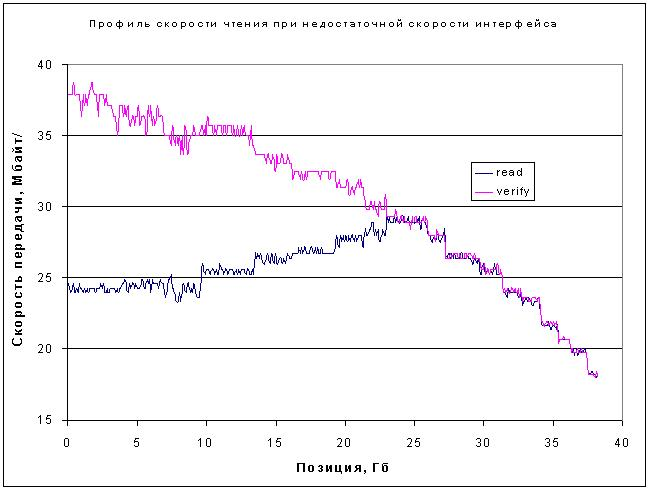
\includegraphics[width=0.8\textwidth]{graph2.png}
    \caption{}
    \label{}
\end{figure}

Для современных дисков время доступа составляет порядка 15 мс, а устоявшаяся скорость линейной передачи данных -- порядка 30 Мбайт/с. Нетрудно заметить, что за время поиска можно было бы считать или записать почти полмегабайта информации. Однако, реально информация читается чаще всего либо покластерно, т.е. по 4 Кбайта, либо максимальными фрагментами, поддерживаемыми BIOS -- 64 Кбайта. Кроме того, объем однократно считанного фрагмента информации никогда не превышает размера файла (точнее, суммарной длины занимаемых им кластеров), а средний размер файла, как правило, не превосходит нескольких килобайт. Поэтому определяющий вклад в производительность дисковой системы вносит время доступа, а линейная скорость передачи лишь очень незначительно влияет на время выполнения файловых операций. Даже при записи или чтении одного длинного файла в однозадачной системе реальная скорость обмена оказывается существенно, иногда в разы, ниже установившейся скорости накопителя.

\begin{figure}[H]
    \centering
    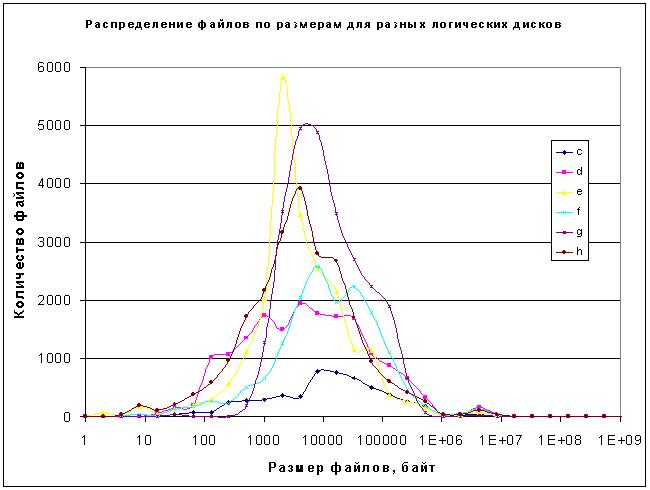
\includegraphics[width=0.88\textwidth]{graph3.png}
    \caption{}
    \label{}
\end{figure}

Время доступа определяется скоростью вращения диска, конструкцией механизма позиционирования головки, а также линейными размерами, на которые необходимо совершить перемещение, т. е. диаметром пластин. Установившаяся скорость обмена в основном зависит от плотности записи и скорости вращения. Вряд ли следует ожидать существенного увеличения скорости вращения пластин, поэтому в перспективе вряд ли можно надеяться на заметный прирост эксплуатационной производительности жестких дисков.

Уменьшение времени доступа возможно в основном за счет уменьшения диаметра пластин, что делает возможным как увеличение скорости вращения, так и уменьшения времени позиционирования. Однако этот подход ведет к радикальному уменьшению емкости накопителя. И хотя первых жесткий диск имел пластины диаметром 24 дюйма, первый, применяемый в персональном компьютере – около 5 (формфактор корпуса 5.25”), а современные – около 3 (а скоростные накопители SCSI при формфакторе корпуса 3.5" имеют уменьшенные пластины), вряд ли в ближайшее время можно ожидать повального перехода на 2.5-дюймовые накопители. Скорее уж революцию во времени доступа следует связывать с переходом на твердотельные накопители.

Наиболее эффективным средством повышения производительности дисковой системы является кэширование, т.е. хранение в оперативной памяти наиболее часто используемых данных с жесткого диска. Ведь для доступа к определенному байту, расположенному на диске, требуется около 15 мс, а к расположенному в оперативной памяти -- порядка 0.1 мкс. Даже однокластерное (буфер 4 Кбайта) кэширование при построчном чтении текстового файла с длиной строки 80 символов приведет к уменьшению времени считывания в 50 раз. Увеличение объема буфера еще более ускорит этот процесс, поэтому, во-первых, сами накопители содержат буфер объемом, как правило, от 2 до 8 Мбайт, а во-вторых, кэширование производится на уровне ОС.


\section{Интерфейс}

В настоящее время для жестких дисков (не считая части накопителей для ноутбуков, носимой аппаратуры, а также внешних моделей) используются два параллельных интерфейса, разработанных в 80-х годах прошлого века: IDE (ATA) и SCSI.

IDE более демократичен. Основная нагрузка в нем ложится на контроллер устройства. Первые его модификации работали в режиме программируемого ввода/вывода (PIO) и были ограничены скоростями от 3 до 16 Мбайт/с. Впрочем, внешние контроллеры часто еще сильнее ``тормозились'' шиной ISA. Реально даже на шине PCI от такого контроллер не удавалось добиться скорости обмена выше 8-9 Мбайт/с. Тогда был использован поддерживаемый PCI механизм прямого обмена с памятью (UDMA), в результате чего максимальная скорость выросла до 33, 66 или 100 Мбайт/с в зависимости от разновидности интерфейса (а компания Maxtor выпускает даже диски UDMA133).

SCSI обладает как более широкими возможностями, так и более высокой ценой. К этому интерфейсу можно подключать не только дисковые накопители, но также ленточные накопители, сканеры, принтеры и т. д. Кроме того, он позволяет одновременно работать нескольким устройствам, что снижает нагрузку на центральный процессор. Диапазон скоростей, поддерживаемых SCSI простирается от 5 до 320 Мбайт/с. В перспективе планируется увеличение скорости обмена до 640 Мбайт/с.

Последнее время IDE существенно потеснил SCSI. Особенно после введения режима UDMA, в результате чего сильно снизилась нагрузка на процессор, и исчезло основное преимущество SCSI перед IDE. Одновременно появление USB стало вытеснить SCSI из низкоскоростных устройств, таких как сканеры и принтеры.

Дальнейшее увеличение скорости при использовании параллельных интерфейсов уже упирается в очень серьезные проблемы по синхронизации линий передачи данных, поэтому, как представляется, будущее за последовательными интерфейсами.

В настоящее время активно идет разработка последовательного варианта интерфейса IDE -- Serial ATA. К контроллеру каждый накопитель будет подключаться своим 7-жильным кабелем. Первый намеченный рубеж скорости -- 150 Мбайт/с, на очереди -- 300 Мбайт/с. Эти интерфейсы, несмотря на существенное аппаратное различие будут программно совместимы с существующим сейчас параллельным IDE.

Определенные разработки намечены и для совершенствования интерфейса SCSI. Здесь также намечен переход на последовательный интерфейс, а также на существенное снижение стоимости вследствие сильной конкуренции со стороны SerialATA.

Для накопителей на жестких дисках помимо рассмотренных могут применяться интерфейсы Compact Flash Type II -- для 1-дюймового накопителя IBM MicroDrive, USB, IEEE1394 (FireWire) -- для внешних устройств и Fibre Channel -- для наиболее производительных серверов.

\section{Область применения}

Область применения жестких дисков довольно широка:
\begin{enumerate}
    \item \textit{Карты расширения} -- вид компьютерных комплектующих: печатная плата, которую устанавливают в слот расширения материнской платы компьютерной системы с целью добавления дополнительных функций. Платы расширения, необходимые для подключения внешних устройств, могут также называться адаптерами или контроллерами этих устройств.
    \item Системные блоки настольных компьютеров
    \item Ноутбуки
    \item \textit{Цифровые видеорекордеры} -- устройство или приложение для записи видеосигнала и звука в цифровом формате на электронные носители с целью последующего воспроизведения. В качестве носителей могут применяться жёсткие диски, оптические диски, твердотельные накопители, USB-флеш-накопители, карты памяти.
    \item \textit{RAID-массивы} -- технология виртуализации данных для объединения физических дисковых устройств в логический модуль для повышения отказоустойчивости и производительности.
    \item \textit{Цифровые портативные мультимедийные проигрыватели} -- класс электронных устройств небольших размеров, сочетающих в себе функции сразу нескольких аппаратов. От обычных плееров их часто отличает наличие крупного дисплея. Портативный мультимедийный проигрыватель является дальнейшим развитием портативных устройств воспроизведения и обычно включает в себя аудио- и видеоплеер, радиоприёмник, диктофон, с их помощью можно просматривать изображения и видео. Существуют также модели со встроенным ТВ-тюнером и возможностью работы с картами памяти, например, IRiver B20 или Cowon iAudio D2. Самые функциональные модели также имеют сенсорный дисплей, Wi-fi, Bluetooth и операционную систему Android. Начиная с 2011 года, данный класс устройств начал быстро исчезать в связи с развитием технологий и распространением смартфонов, которые, имея те же функции, обладают ещё и функцией связи,а также стремительно дешевеют.
    \item Поскольку в настоящее время DVD-приводы в ноутбуках и моноблоках неактуальны, очень часто туда вставляют HDD в специальном адаптере
\end{enumerate}


\section{Технология записи данных и методы записи и хранения}

Принцип работы жёстких дисков похож на работу магнитофонов (как бы это странно не звучало). Рабочая поверхность диска движется относительно считывающей головки (например, в виде катушки индуктивности с зазором в магнитопроводе). При подаче переменного электрического тока (при записи) на катушку головки возникающее переменное магнитное поле из зазора головки воздействует на ферромагнетик поверхности диска и изменяет направление вектора намагниченности доменов в зависимости от величины сигнала. При считывании перемещение доменов у зазора головки приводит к изменению магнитного потока в магнитопроводе головки, что приводит к возникновению переменного электрического сигнала в катушке за счёт электромагнитной индукции. С конца 1990-х на рынке устройств хранения информации начали применяться головки на основе эффекта гигантского магнитного сопротивления (ГМС). С начала 2000-х головки на основе эффекта ГМС стали заменяться на головки на основе туннельного магниторезистивного эффекта (в них изменение магнитного поля приводит к изменению сопротивления в зависимости от изменения напряжённости магнитного поля; подобные головки позволяют увеличить вероятность достоверности считывания информации, особенно при больших плотностях записи информации). В 2007 году устройства на основе туннельного магниторезистивного эффекта с оксидом магния (эффект открыт в 2005 году) полностью заменили устройства на основе эффекта ГМС.

\subsection{Методы записи данных на диск}

\begin{enumerate}
    \item \textbf{Метод продольной записи} -- биты информации записываются с помощью маленькой головки, которая, проходя над поверхностью вращающегося диска, намагничивает миллиарды горизонтальных дискретных областей -- доменов. При этом вектор намагниченности домена расположен продольно, то есть параллельно поверхности диска. Каждая из этих областей является логическим нулём или единицей, в зависимости от направления намагниченности. Максимально достижимая при использовании данного метода плотность записи составляет около 23 Гбит/см$^2$. К 2010 году этот метод был практически вытеснен методом перпендикулярной записи.
    \item \textbf{Метод перпендикулярной записи} -- технология, при которой биты информации сохраняются в вертикальных доменах. Это позволяет использовать более сильные магнитные поля и снизить площадь материала, необходимую для записи 1 бита. Предыдущий метод записи, параллельно поверхности магнитной пластины, привёл к тому, что в определённый момент инженеры упёрлись в «потолок» -- дальше увеличивать плотность информации на дисках было невозможно. И тогда вспомнили о другом способе записи, который был известен ещё с 1970-х годов. Плотность записи при этом методе резко возросла — более чем на 30\% ещё на первых образцах (на 2009 год -- 400 Гбит/дюйм$^2$, или 62 Гбит/см$^2$). Теоретический предел отодвинулся на порядки и составляет более 1 Тбит/дюйм$^2$. Жёсткие диски с перпендикулярной записью стали доступны на рынке с 2006 года. Винчестеры продолжают тенденцию на увеличение ёмкости, вмещая до 10-14 терабайт и применяя в дополнение к PMR такие технологии, как заполнение гелием корпусов, SMR, HAMR/MAMR.
    \item Одним из довольно перспективных методов записи информации является \textbf{метод черепичной магнитной записи}. Этот метод (англ. Shingled magnetic recording, SMR) был реализован в начале 2010-х годов. В нём используется тот факт, что ширина области чтения меньше, чем ширина записывающей головки. Запись дорожек в этом методе производится с частичным наложением в рамках групп дорожек (пакетов). Каждая следующая дорожка пакета частично закрывает предыдущую (подобно черепичной кровле), оставляя от неё узкую часть, достаточную для считывающей головки. По своей специфике она радикально отличается от более популярных технологий записи CMR и PMR.
    \item Имеет место также \textbf{метод тепловой магнитной записи}. Это -- гибридная технология записи информации, комбинирующая магнитное чтение и магнитооптическую запись. Метод тепловой магнитной записи (англ. heat-assisted magnetic recording, HAMR) остаётся перспективным, продолжаются его доработки и внедрение. В этом методе используется точечный подогрев диска, который позволяет головке намагничивать очень мелкие области его поверхности. После того, как диск охлаждается, намагниченность «закрепляется». На 2009 год были доступны только экспериментальные образцы, плотность записи которых составляла 150 Гбит/см$^2$. Специалисты Hitachi называют предел для этой технологии в 2,3-3,1 Тбит/см$^2$, а представители Seagate Technology -- 7,75 Тбит/см$^2$
    \item Теперь взглянем на ситуацию по другому - а что, если развивать не метод записи, а технологию хранения, чтобы ускорить процесс записи? В этом случае нам будет интересен \textbf{``Структурированный носитель данных''} (англ. bit-patterned media) -- перспективная технология хранения данных на магнитном носителе, использующая для записи данных массив одинаковых магнитных ячеек, каждая из которых соответствует одному биту информации, в отличие от современных технологий магнитной записи, в которых бит информации записывается на нескольких магнитных доменах.
\end{enumerate}

% Раздел "Заключение"
\conclusion

В нынешнее время -- информационную эру -- когда каждый год развитие технологий многократно ускоряется, а информация теперь является одним из самых важных ресурсов (если, может быть, не самым важным), необходимо также трепетно относится к способу хранения, передачи и записи этой самой драгоценной информации. Поэтому определенно стоит уделять внимание вопросу улучшения способов хранения данных, и, соответственно, улучшению носителей данных, увеличению объема хранения, скорости записи и надежности - развивать перспективные технологии хранения, экспериментировать, соединяя различные методы технологий, и так далее. Нельзя недооценивать то, что позволяет нам хранить кладезь знаний -- напротив, нужно подвергать это особому вниманию.


%Библиографический список, составленный вручную, без использования BibTeX

\begin{thebibliography}{99}
    \bibitem{obzor} https://itbukva.com/promo/14881-gde-khranit-informatsiyu-obzor-sovremennykh-tsifrovykh-nositelej.html
    \bibitem{smarthdd} https://smarthdd.com/rus/help.htm
    \bibitem{hdd_inside} https://www.youtube.com/watch?v=KftyBnuDBII
    \bibitem{Andrianov} Андрианов С. Основные сведения о жёстких дисках / С. Андрианов // MorePC. — 2002. — 21 июля.
    \bibitem{Vishnyakova} Вишнякова Н. Устройство и принцип работы жёсткого диска / Н. Вишнякова // Компьютер с нуля. — 2012. — 26 марта.
    \bibitem{history_hdd} https://interteam.com.ua/istoriya-zhestkix-diskov-ot-pervogo-hdd-do-ssd/
\end{thebibliography}

%Библиографический список, составленный с помощью BibTeX
%\bibliographystyle{mdpi}
% \bibliographystyle{gost780uv}
% \bibliography{thesis}

% Окончание основного документа и начало приложений
% Каждая последующая секция документа будет являться приложением

% \appendix

\end{document}
